\section{Model}\label{model}

\subsection{Delegates}

Figure \ref{Delegate} shows the number of delegates awarded after each primary/caucus per candidate. The results are displayed for each state until Super Tuesday.

\begin{figure}[H]
    \centering
    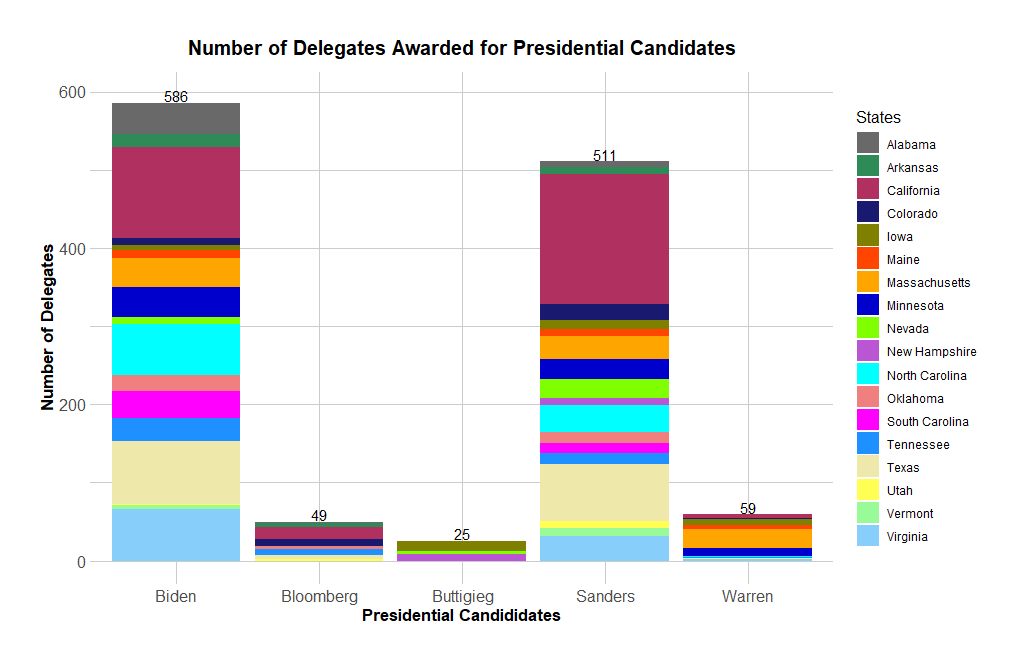
\includegraphics[width=0.9\textwidth]{figures/Delegate.png}
    \caption{Candidate's Delegate Distribution}
    \label{Delegate}
\end{figure}

\subsection{Polling}

Figures \ref{Updated-Polling-Data-1} to \ref{scatter-all-linear} show the general polling results over time from a large number of different pollsters. Figures \ref{Updated-Polling-Data-1}, \ref{A-rated-polls}, and \ref{All-rated-polls} contain aggregated polling data, where polls conducted on the same day have been averaged out. Figures \ref{scatter-A-rated}, \ref{scatter-all}, and \ref{scatter-all-linear} contain scatter plots of the various polling results and a fitted regression line.

\begin{figure}[H]
    \centering
    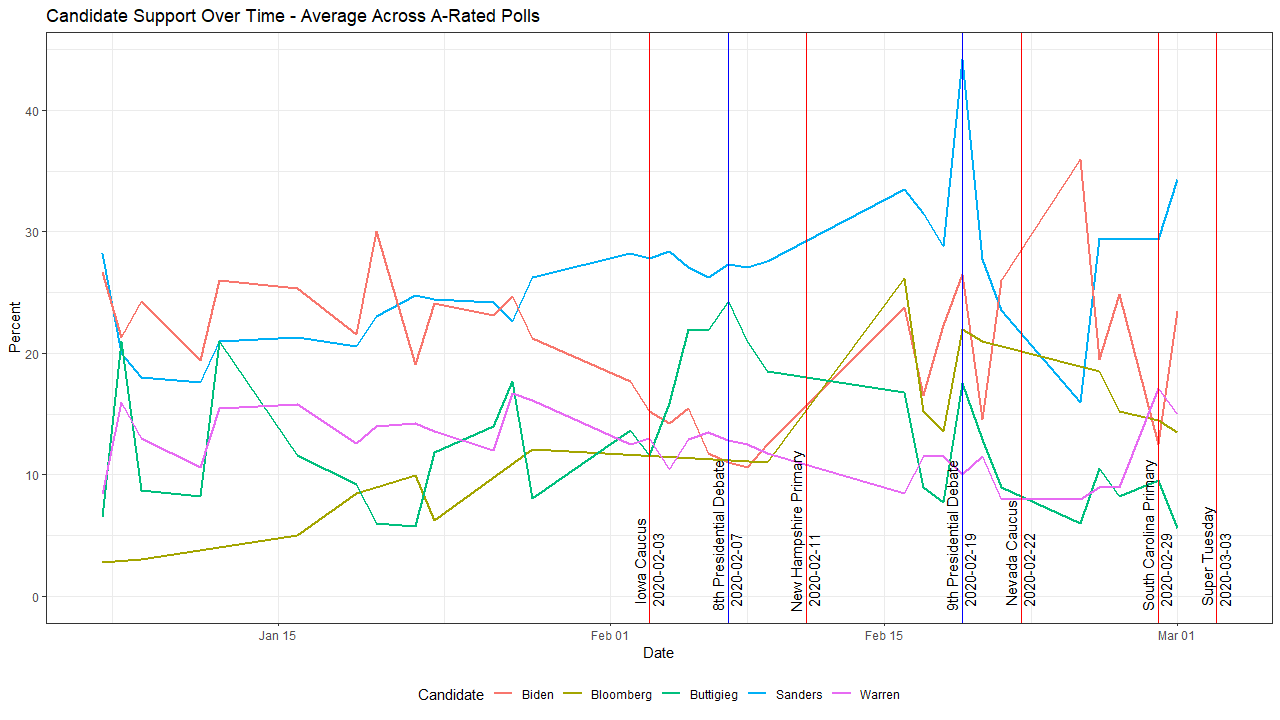
\includegraphics[width=0.9\textwidth]{figures/long-A-rated-polls.png}
    \caption{A-Rated Polling Data - Jan. 1 through Mar. 3}
    \label{Updated-Polling-Data-1}
\end{figure}

\begin{figure}[H]
    \centering
    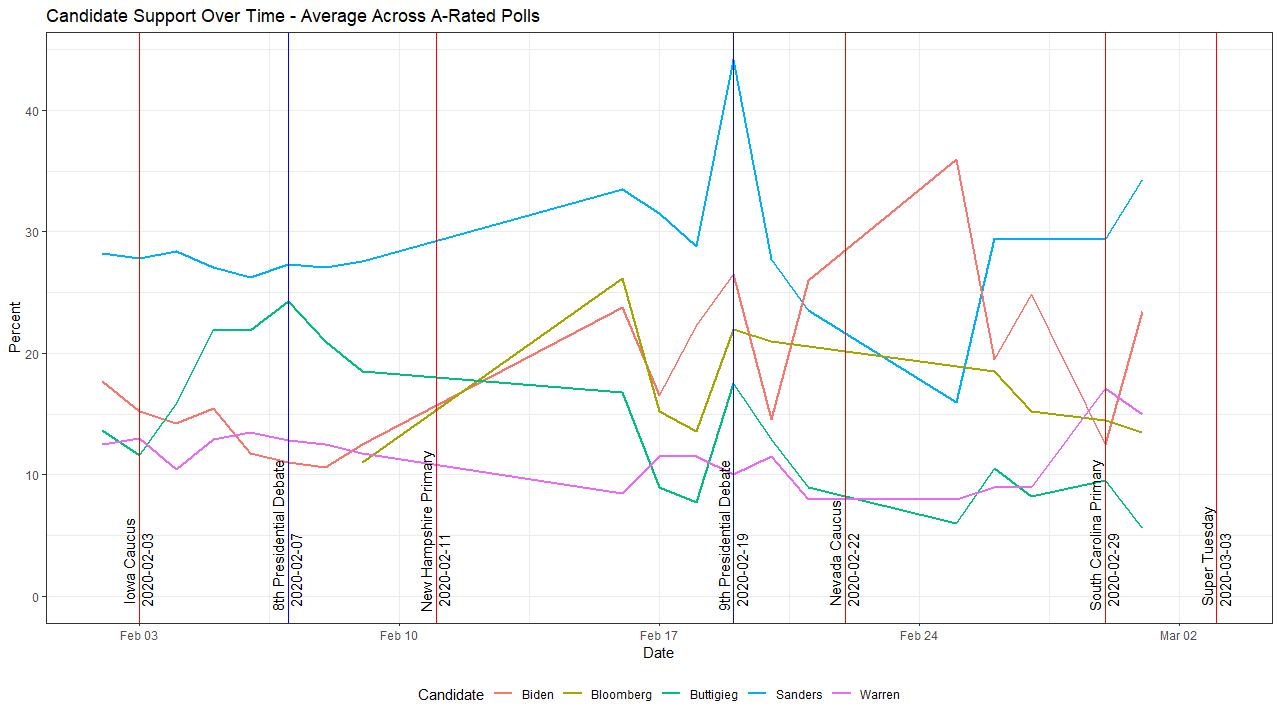
\includegraphics[width=0.9\textwidth]{figures/A-rated-polls.png}
    \caption{A-Rated Polling Data - Feb. 1 through Mar. 3}
    \label{A-rated-polls}
\end{figure}

\begin{figure}[H]
    \centering
    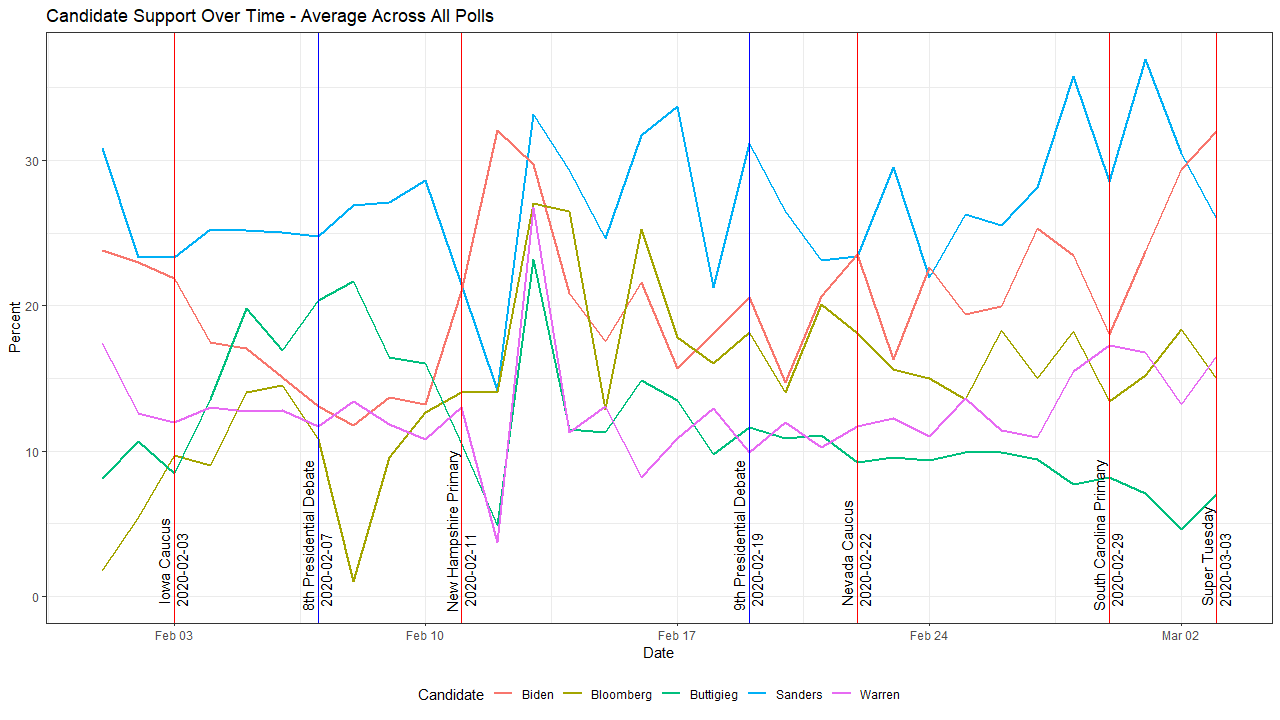
\includegraphics[width=0.9\textwidth]{figures/All-rated-polls.png}
    \caption{All Polling Data - Feb. 1 through Mar. 3}
    \label{All-rated-polls}
\end{figure}

\begin{figure}[H]
    \centering
    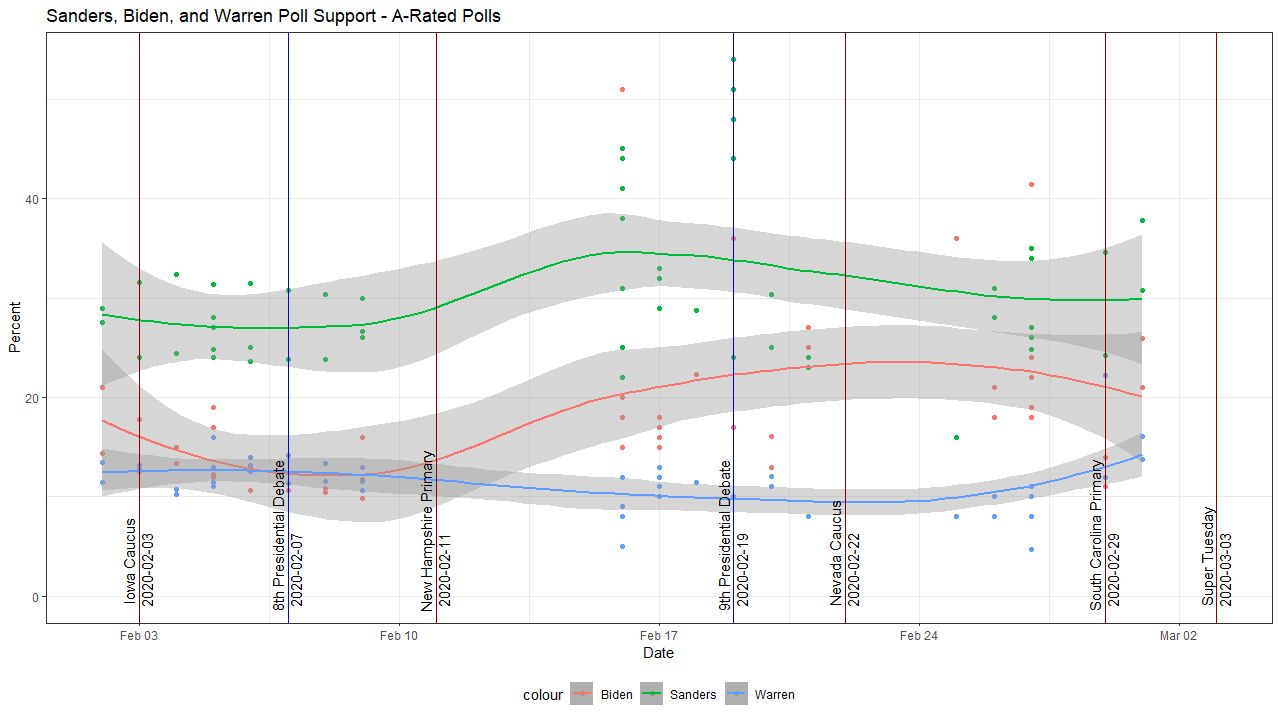
\includegraphics[width=0.9\textwidth]{figures/scatter-A-rated.png}
    \caption{A-Rated Polling Data - Fitted Regression - Feb. 1 through Mar. 3}
    \label{scatter-A-rated}
\end{figure}

\begin{figure}[H]
    \centering
    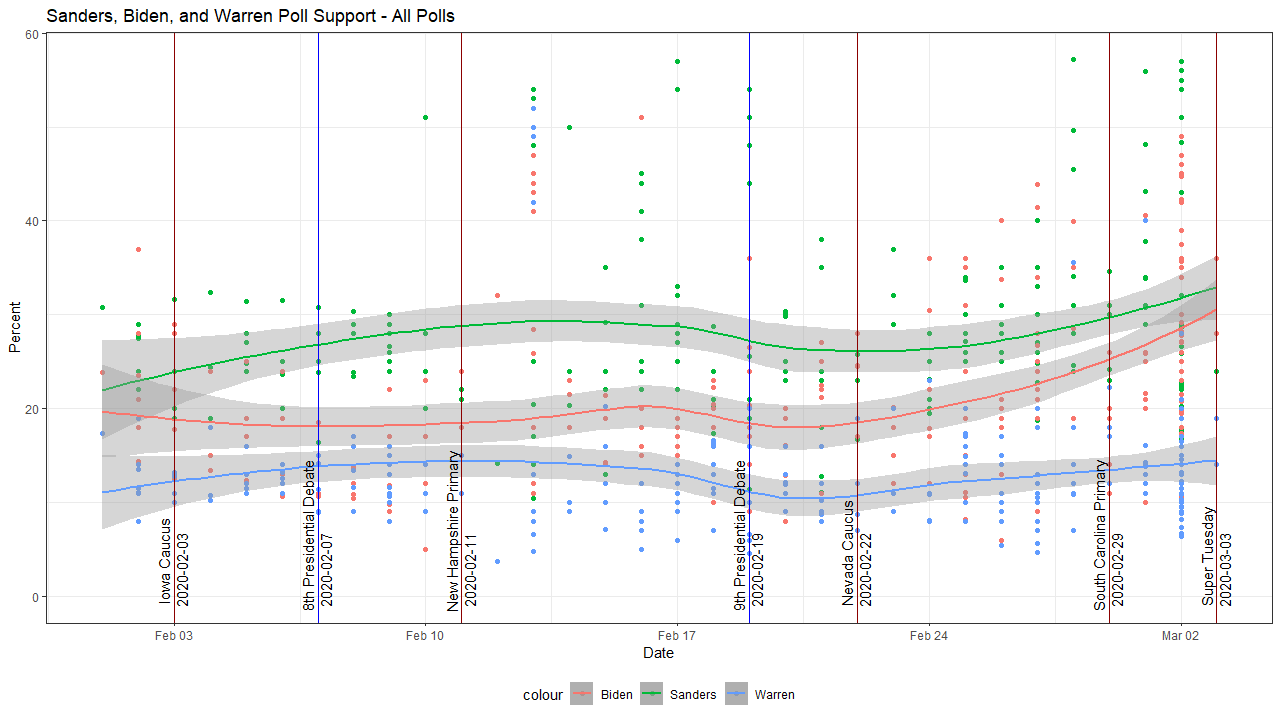
\includegraphics[width=0.9\textwidth]{figures/scatter-all.png}
    \caption{All Polling Data - Fitted Regression - Feb. 1 through Mar. 3}
    \label{scatter-all}
\end{figure}

\begin{figure}[H]
    \centering
    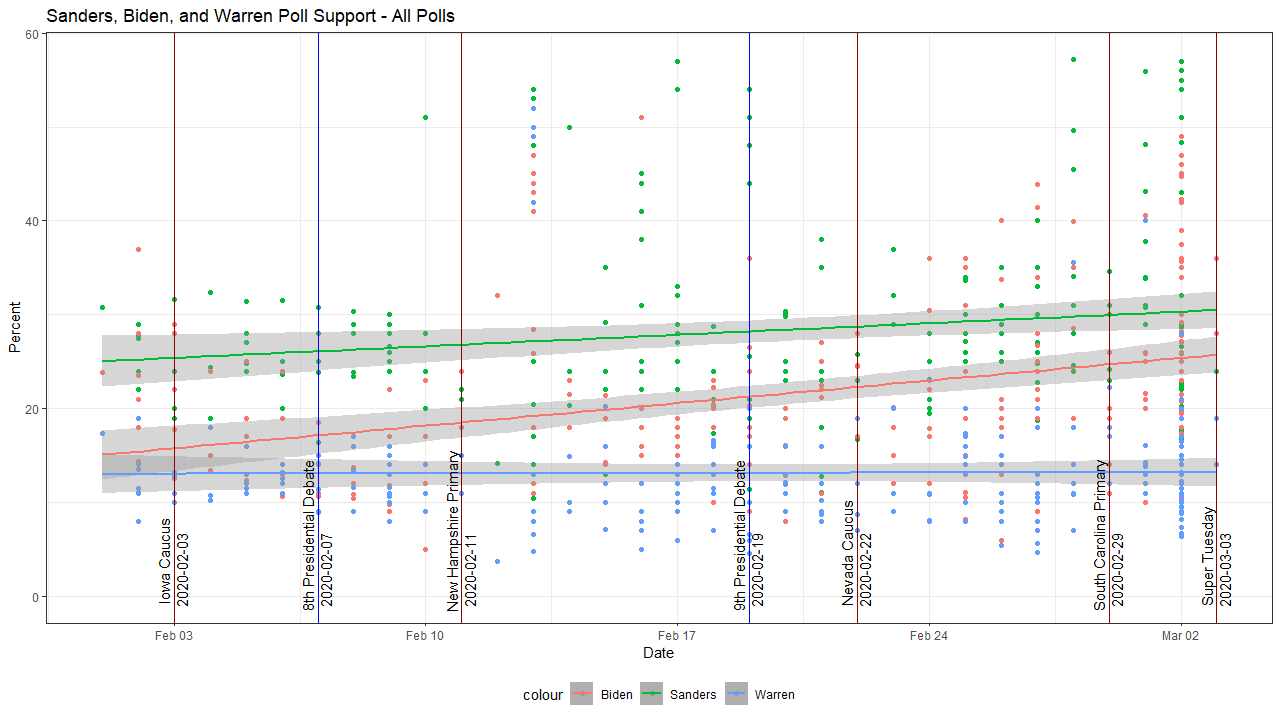
\includegraphics[width=0.9\textwidth]{figures/scatter-all-linear.png}
    \caption{All Polling Data - Linear Regression - Feb. 1 through Mar. 3}
    \label{scatter-all-linear}
\end{figure}

\subsection{Spending}

Figures \ref{MoneyspendinAds} to \ref{Nevada} show the amount of money spent on advertisements state wise (Iowa, New Hampshire and Nevada).

\begin{figure}[H]
    \centering
    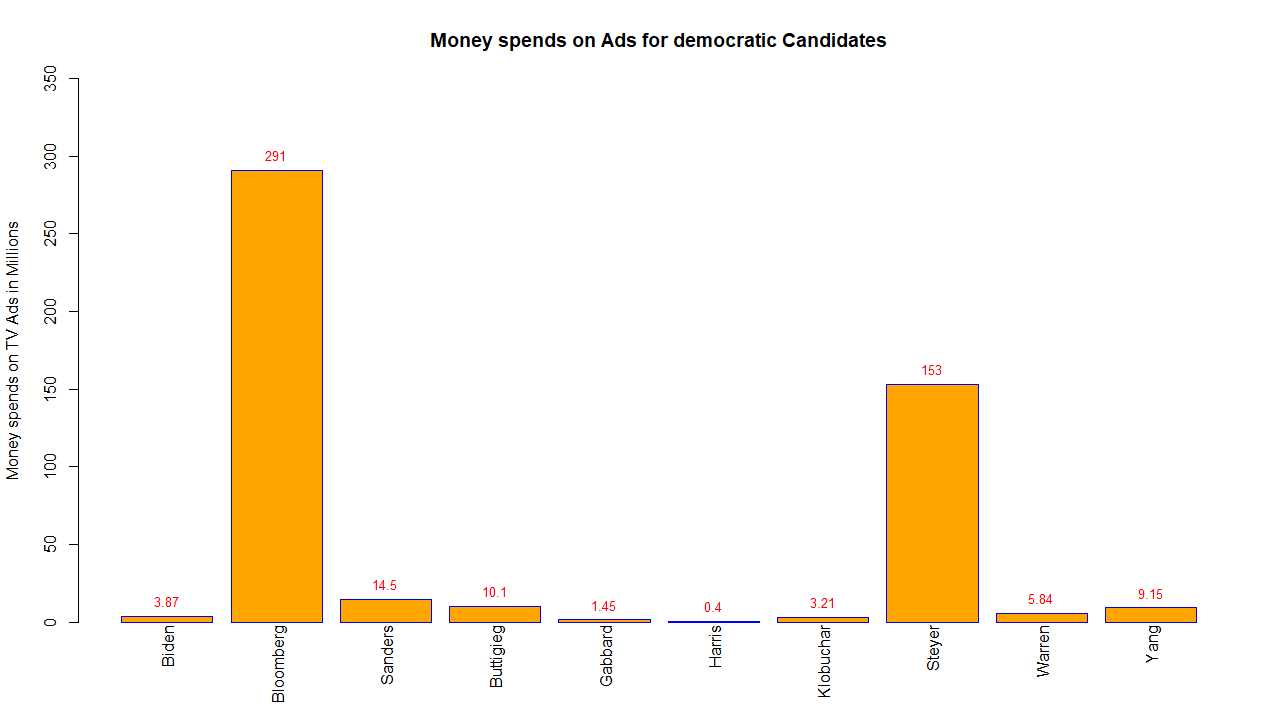
\includegraphics[width=0.9\textwidth]{figures/MoneyspendinAds.png}
    \caption{Candidate's Total TV Ad Spending}
    \label{MoneyspendinAds}
\end{figure}

\begin{figure}[H]
    \centering
    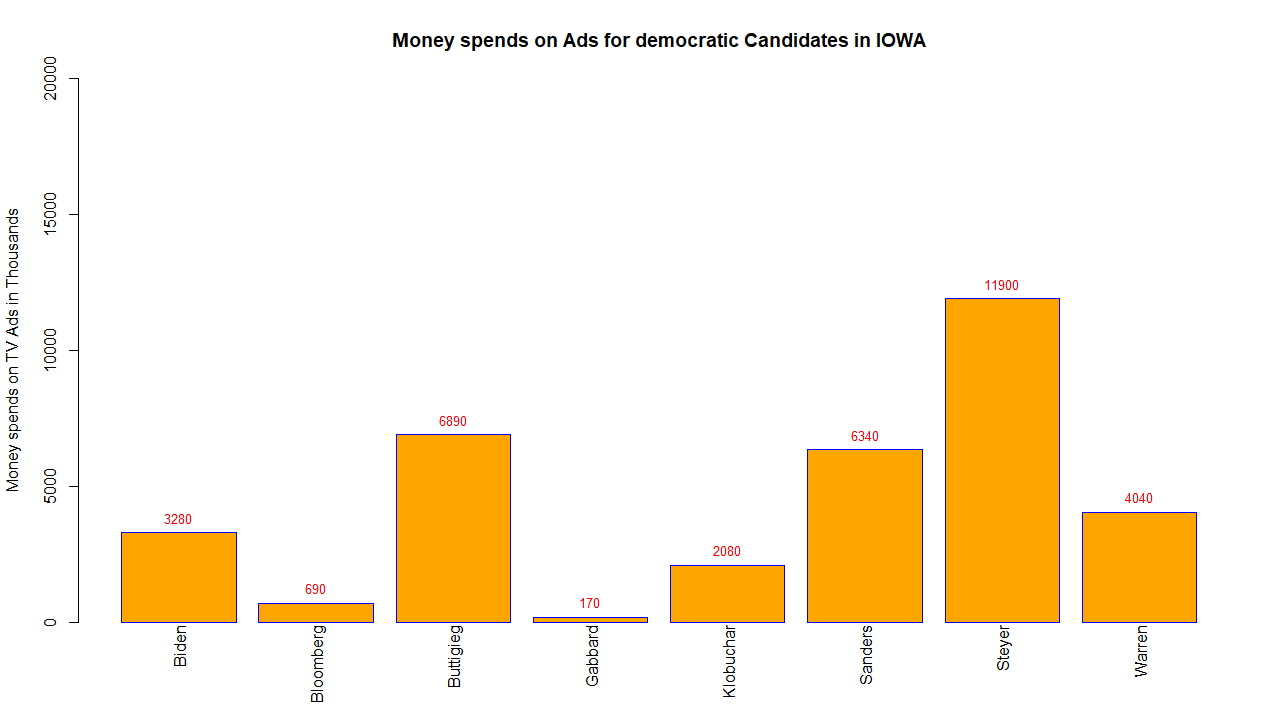
\includegraphics[width=0.9\textwidth]{figures/IOWA.png}
    \caption{Candidate's TV Ad Spending - Iowa}
    \label{IOWA}
\end{figure}

\begin{figure}[H]
    \centering
    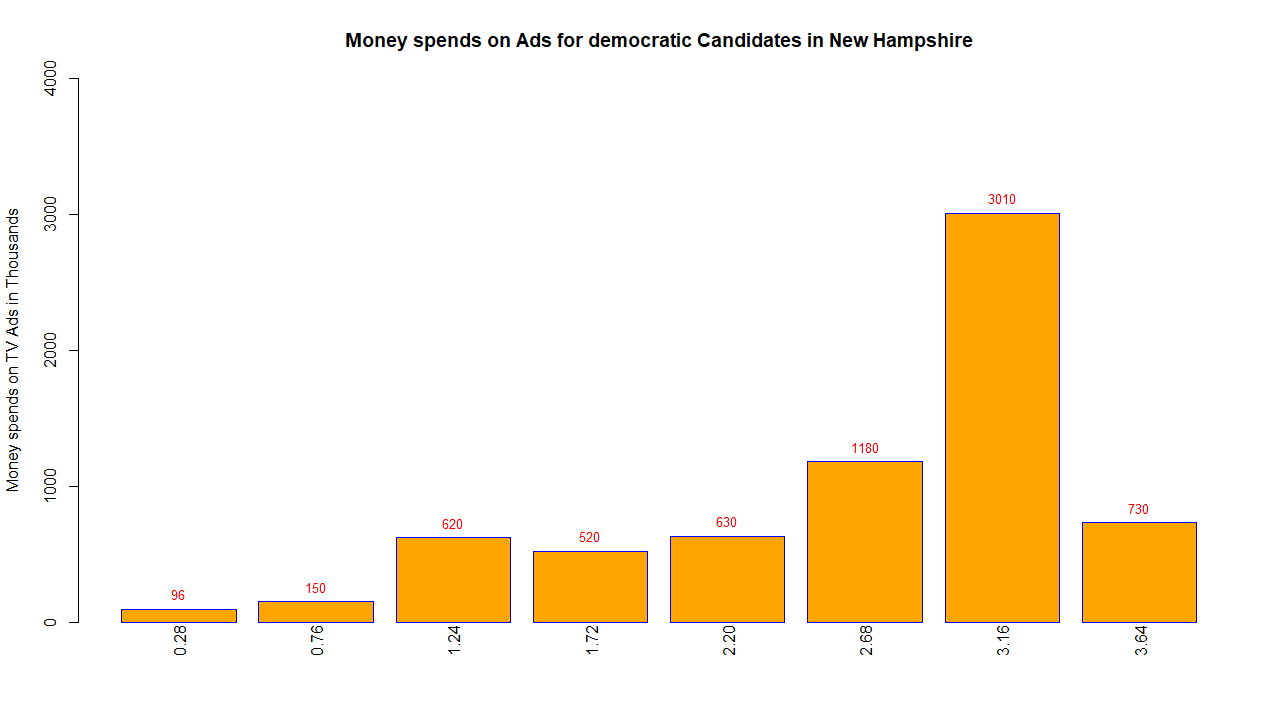
\includegraphics[width=0.9\textwidth]{figures/Newhampshire.png}
    \caption{Candidate's TV Ad Spending - New Hampshire}
    \label{Newhampshire}
\end{figure}

\begin{figure}[H]
    \centering
    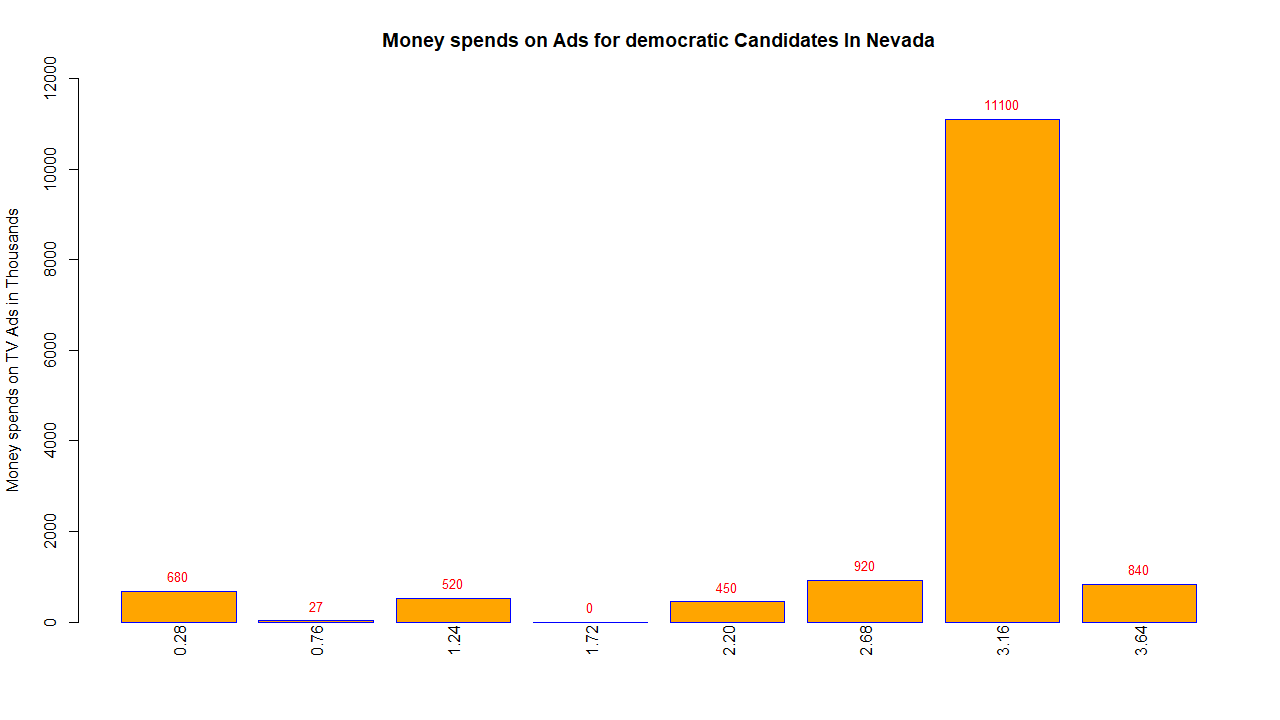
\includegraphics[width=0.9\textwidth]{figures/Nevada.png}
    \caption{Candidate's TV Ad Spending - Nevada}
    \label{Nevada}
\end{figure}

\subsection{Funding}

Figures \ref{Total} to \ref{Others} shows funding from small and big donors,  self funding and funding from other sources.

\begin{figure}[H]
    \centering
    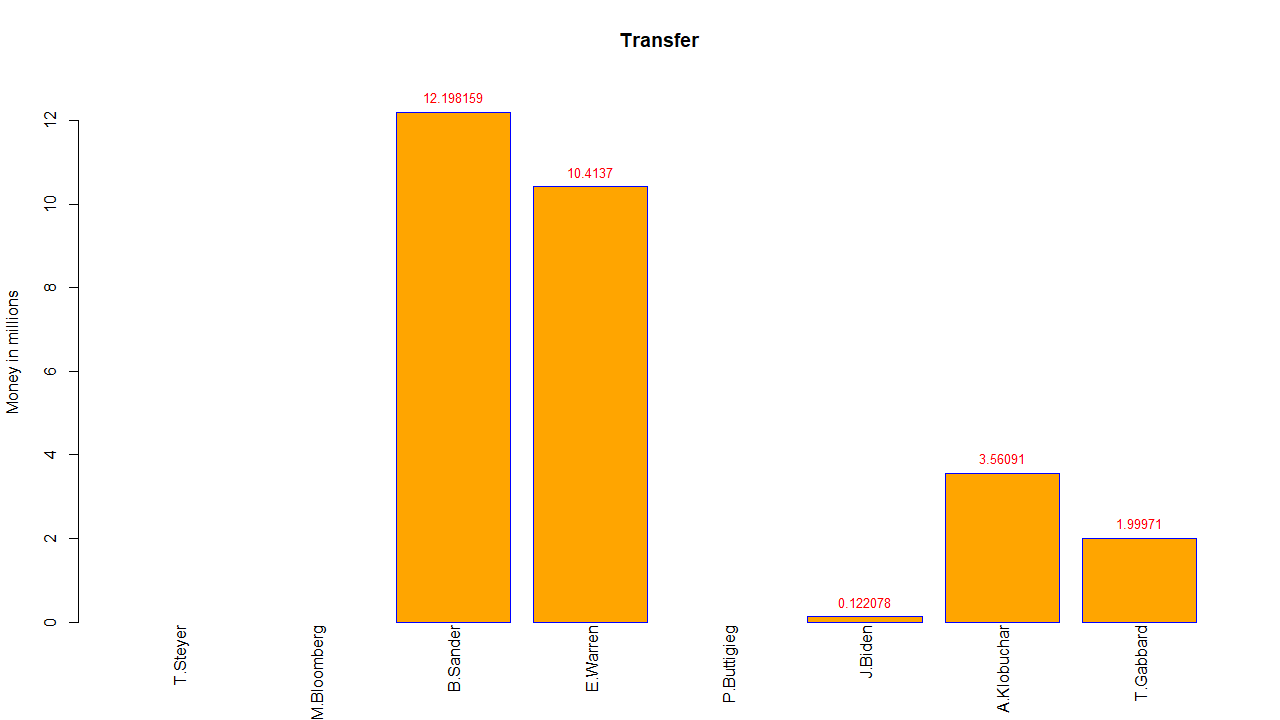
\includegraphics[width=0.9\textwidth]{figures/Total.png}
    \caption{Candidate's Total Funding}
    \label{Total}
\end{figure}

\begin{figure}[H]
    \centering
    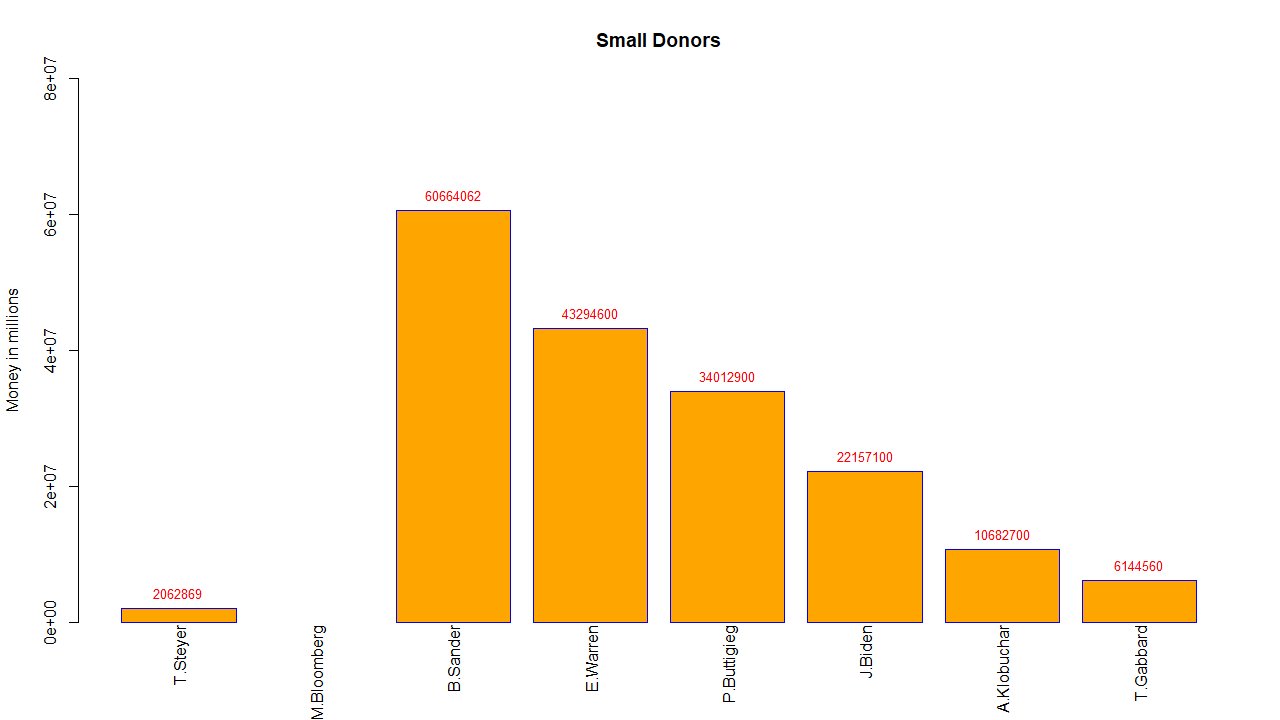
\includegraphics[width=0.9\textwidth]{figures/Small Donors.png}
    \caption{Candidate's Small Donors Funding}
    \label{Small Donors}
\end{figure}

\begin{figure}[H]
    \centering
    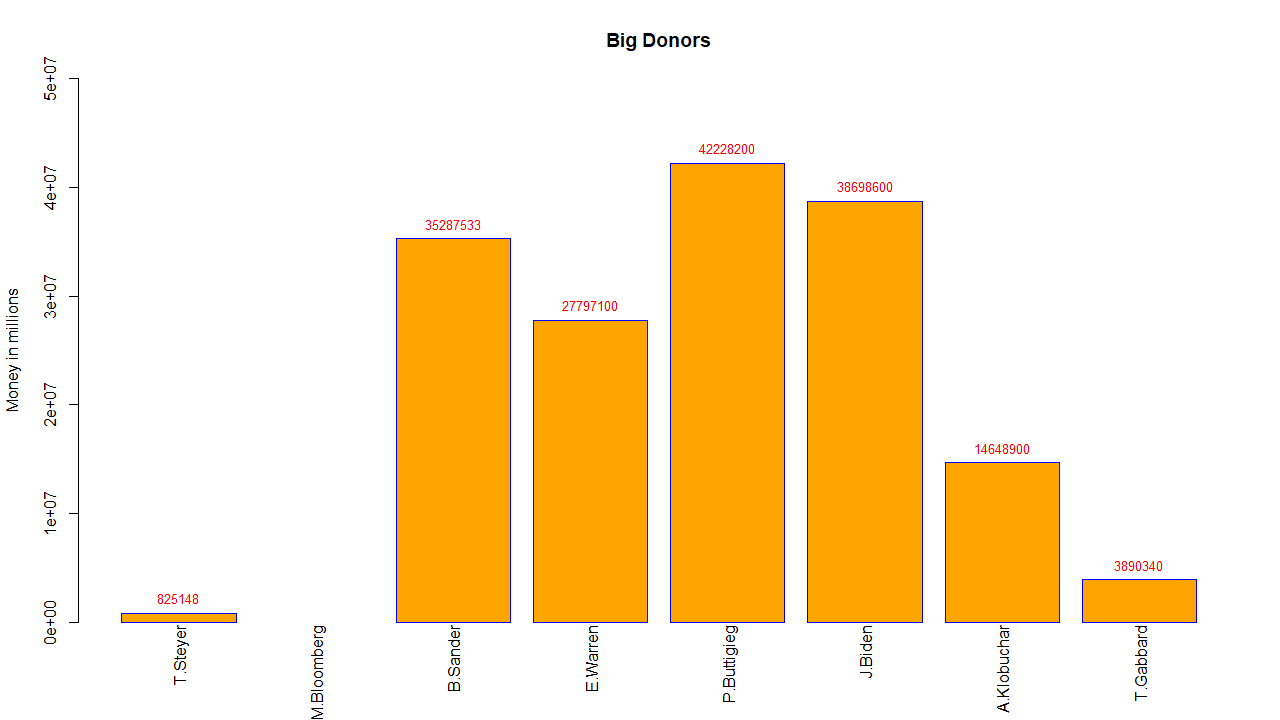
\includegraphics[width=0.9\textwidth]{figures/Bigdonor.png}
    \caption{Candidate's Big donors Funding}
    \label{Bigdonor}
\end{figure}

\begin{figure}[H]
    \centering
    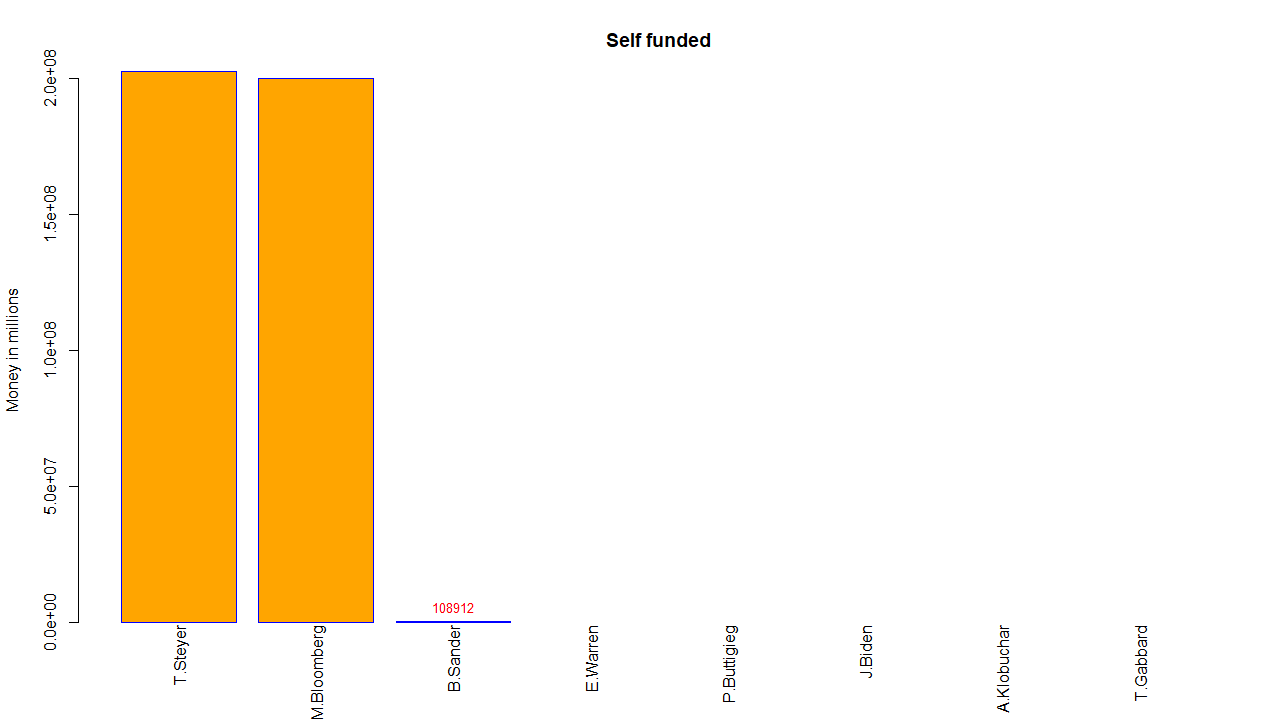
\includegraphics[width=0.9\textwidth]{figures/Selffunnded.png}
    \caption{Candidate's Self Funding}
    \label{Selffunnded}
\end{figure}

\begin{figure}[H]
    \centering
    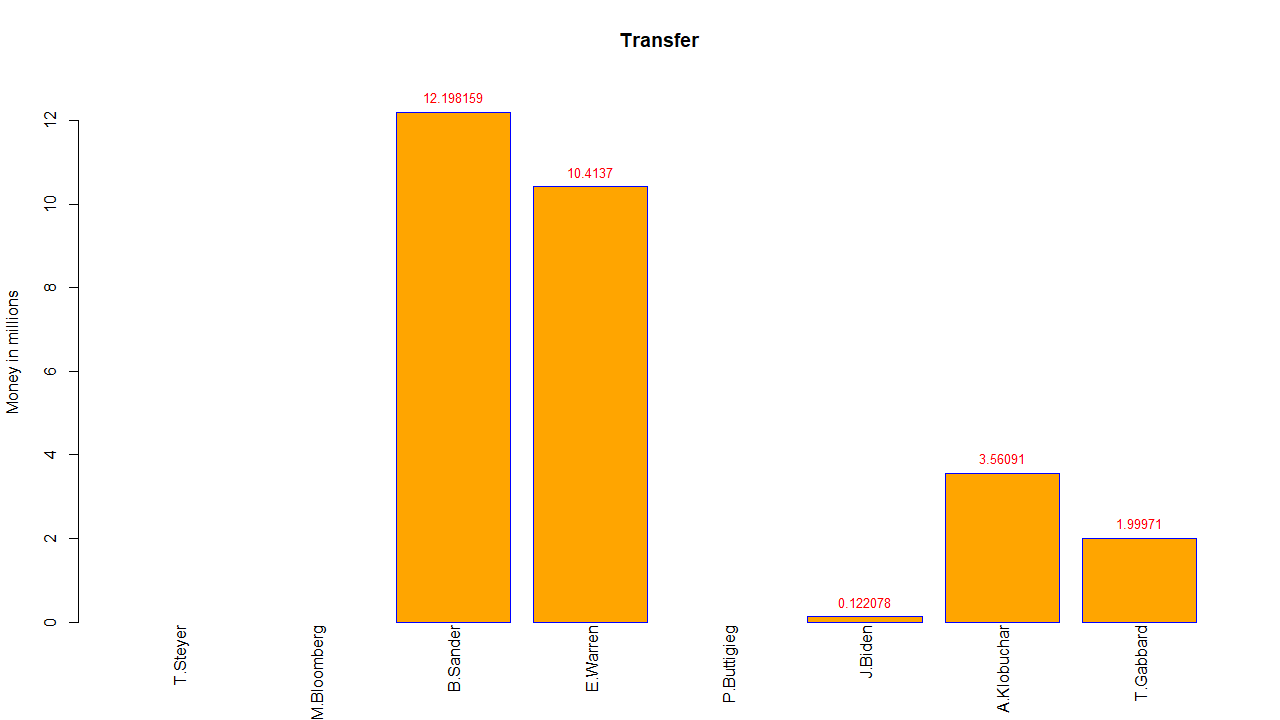
\includegraphics[width=0.9\textwidth]{figures/Transfer.png}
    \caption{Candidate's Transfer Funding}
    \label{Transfer}
\end{figure}

\begin{figure}[H]
    \centering
    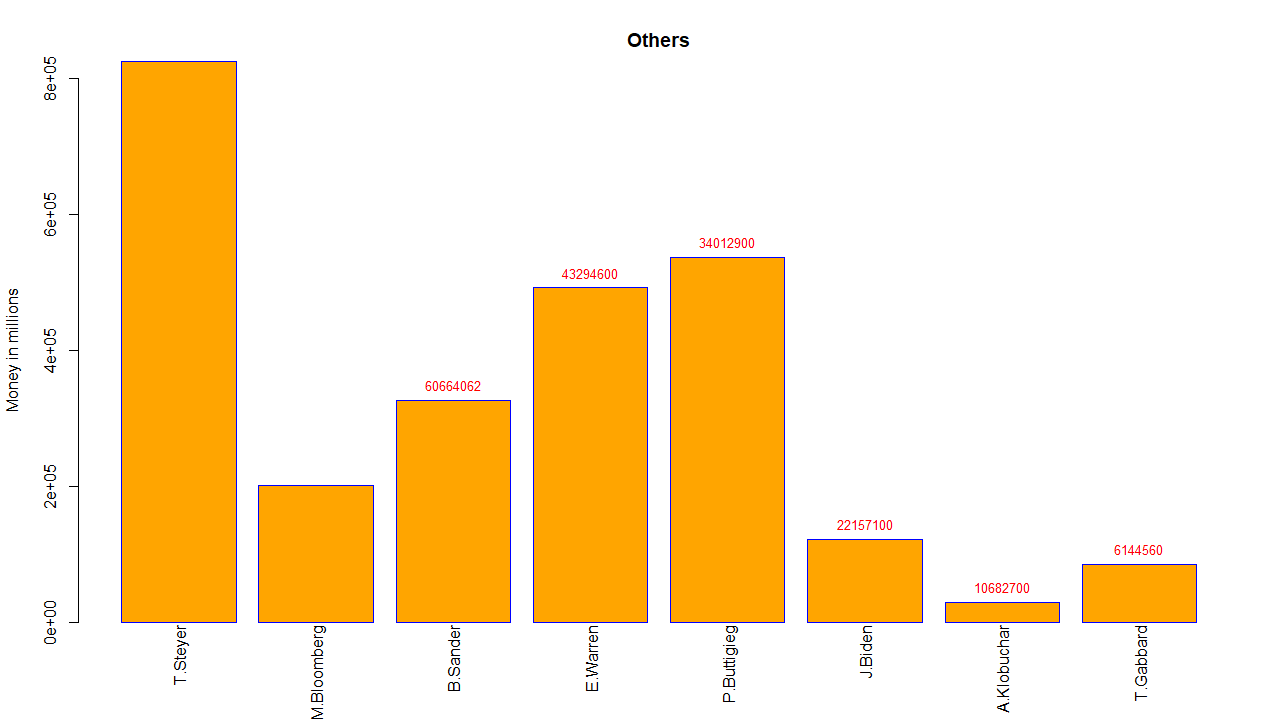
\includegraphics[width=0.9\textwidth]{figures/Others.png}
    \caption{Candidate's Others Sources of Funding}
    \label{Others}
\end{figure}
